\documentclass{article}

% if you need to pass options to natbib, use, e.g.:
% \PassOptionsToPackage{numbers, compress}{natbib}
% before loading nips_2016
%
% to avoid loading the natbib package, add option nonatbib:
% \usepackage[nonatbib]{nips_2016}

%\usepackage{nips_2016}

% to compile a camera-ready version, add the [final] option, e.g.:
 \usepackage[final]{nips_2016}

\usepackage[utf8]{inputenc} % allow utf-8 input
\usepackage[T1]{fontenc}    % use 8-bit T1 fonts
\usepackage{hyperref}       % hyperlinks
\usepackage{url}            % simple URL typesetting
\usepackage{booktabs}       % professional-quality tables
\usepackage{amsfonts}       % blackboard math symbols
\usepackage{nicefrac}       % compact symbols for 1/2, etc.
\usepackage{microtype}      % microtypography
\usepackage{tikz}
\usetikzlibrary{fit,positioning}
\usepackage{amsmath}
\usepackage[round]{natbib}
\usepackage{multirow}
\usepackage{caption}
\usepackage{subcaption}

\title{Transforming Variational Autoencoders}

% The \author macro works with any number of authors. There are two
% commands used to separate the names and addresses of multiple
% authors: \And and \AND.
%
% Using \And between authors leaves it to LaTeX to determine where to
% break the lines. Using \AND forces a line break at that point. So,
% if LaTeX puts 3 of 4 authors names on the first line, and the last
% on the second line, try using \AND instead of \And before the third
% author name.

\author{
  Nathan Kong \\
  University of Toronto\\
  \texttt{nathan.kong@mail.utoronto.ca} \\
  %% examples of more authors
  \And
  Jingyao (Jason) Li \\
  University of Toronto \\
  \texttt{jingyao.li@mail.utoronto.ca}\\
  %% Address \\
  %% \texttt{email} \\
  %% \AND
  %% Coauthor \\
  %% Affiliation \\
  %% Address \\
  %% \texttt{email} \\
  %% \And
  %% Coauthor \\
  %% Affiliation \\
  %% Address \\
  %% \texttt{email} \\
  %% \And
  %% Coauthor \\
  %% Affiliation \\
  %% Address \\
  %% \texttt{email} \\
}

\newcommand{\R}{\mathbb{R}}
\newcommand{\E}{\mathbb{E}}
\newcommand{\bz}{\mathbf{z}}
\newcommand{\bx}{\mathbf{x}}
\newcommand{\bu}{\mathbf{u}}
\newcommand{\bw}{\mathbf{w}}
\newcommand{\given}{\,|\,}
\newcommand{\D[1]}{\mathrm{d}{#1}}
\newcommand{\KL}{\mathbb{D}_{\text{KL}}}
\newcommand{\N}{\mathcal{N}}
\newcommand{\bsig}{\boldsymbol{\sigma}}
\newcommand{\bmu}{\boldsymbol{\mu}}

\begin{document}

\maketitle

\begin{abstract}
In variational inference, the approximate posterior distribution that is chosen is very important.  It
needs to be computationally tractable, yet flexible enough to approximate the true posterior.  In this 
paper, we discuss an application of variational inference in dimensionality reduction.  We experiment
with the variational autoencoder (VAE), which was developed by \citet{KW13}, by comparing two
different variational inference methods.  The first method is the vanilla VAE and the second method
improves variational inference by introducing normalizing flows, developed by \citet{RM15}. Normalizing 
flows increase the complexity of an initial simple distribution, so that more complex true posteriors can
potentially be approximated.
\end{abstract}

\section{Introduction}
Nowadays, with increasingly large amounts of data, making posterior inferences is intractable since 
the evidence in Bayes' Rule consists of a computationally intractable integral.  Stochastic variational 
inference was developed that makes this inference more tractable, by turning the inference problem into
an optimization problem.  In variational inference, an intractable posterior distribution is approximated by
a simpler probability distribution, whose parameters are optimized.  

Unfortunately, extremely complex posterior distributions may not be successfully approximated using 
such simple distributions, so novel methods must be developed to improve the approximations. In this 
paper, we discuss various methods that improve posterior distribution approximations and also compare
the performance of two different methods of variational inference.


\section{Formal Description}
\label{sec:FormalDescription}

\begin{figure}[htdp]
\centering
\hspace{1.5em}
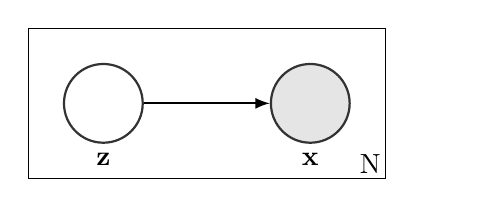
\begin{tikzpicture}
\tikzstyle{main}=[circle, minimum size = 10mm, thick, draw =black!80, node distance = 16mm]
\tikzstyle{connect}=[-latex, thick]
\tikzstyle{box}=[rectangle, draw=black!100]
  \node[main] (z) [label=below:$\bz$] {};
  \node[main, fill = black!10] (x) [right=of z,label=below:$\bx$] { };
  \path (z) edge [connect] (x);
  \node[rectangle, inner sep=0mm, fit= (z) (x),label=below right:N, xshift=13mm] {};
  \node[rectangle, inner sep=4.4mm,draw=black!100, fit= (z) (x)] {};
\end{tikzpicture}
\caption{Probabilistic graphical model with latent variables, $\bz$, and observed variables, $\bx$.}
\label{fig:problem_pgm}
\end{figure}

From a probabilistic graphical model perspective, we have a latent space, governed by $\bz$,
and an observed space, which are our data, $\bx$.  The observed variables depend on the
latent variables.  Figure \ref{fig:problem_pgm} illustrates this model.  Using this framework,
the joint density is: $p(\bx,\bz) = p(\bx \given \bz)\,p(\bz)$. $p(\bz)$ is the prior over the latent 
variables and $p(\bx \given \bz)$ is the likelihood of the data given the latent variables.

\subsection{Variational Lower Bound}
In order to obtain the marginal likelihood $p(\bx)$, we must integrate over $\bz$, which is intractable.  
So, a posterior distribution, $q(\bz \given \bx)$, is introduced allowing us to obtain a lower bound on 
the marginal likelihood:
\begin{align}
	\log p(\bx) &= \log\int_{\bz} p(\bx \given \bz)\,p(\bz)\,\D[\bz] \\
			&= \log\int_{\bz} \frac{q(\bz \given \bx)}{q(\bz \given \bx)}p(\bx \given \bz)\,p(\bz)\,\D[\bz] \\
			&= \log \left(\E_q\left[\frac{p(\bx, \bz)}{q(\bz \given \bx)}\right]\right) \label{eq:evid} \\
			&\geq \E_q\left[\log p(\bx,\bz)\right] - \E_q\left[\log q(\bz \given \bx)\right] \label{eq:pq_lb} \\
			&= \log p(\bx) - \KL\left[q(\bz \given \bx) \,||\, p(\bz \given \bx)\right] \label{eq:KL_evid} \\
			&= -\KL\left[q(\bz \given \bx) \,||\, p(\bz)\right] + \E_{q(\bz \given \bx)}\left[\log p(\bx \given \bz)\right] \label{eq:ELBO}
\end{align}

Equation \ref{eq:pq_lb} follows from Equation \ref{eq:evid} by applying Jensen's inequality.  Equation 
\ref{eq:ELBO} is known as the variational lower bound, which we want to maximize.  Note that from
Equation \ref{eq:KL_evid}, maximizing the lower bound minimizes the Kullback-Leibler (KL) divergence 
between the approximate posterior and the true posterior and maximizes the marginal likelihood since
the KL divergence is always positive.  We want $q(\bz \given \bx)$ to be computationally tractable, but
flexible enough to be able to match $p(\bz \given \bx)$ such that the KL divergence is close to 0.

\subsection{Vanilla VAE}

In an autoencoder, there are two main stages: the encoder stage and the decoder stage, which are
both neural networks.  The input to the encoder, or recognition, stage is the high dimension feature 
vector that we want to reduce into a space with lower dimensionality.  In a VAE, the output of the 
encoder stage are parameters to the approximate posterior, $q(\bz \given \bx)$.  If $q(\bz \given \bx)$
is a Gaussian, the parameters that are output would be the mean, $\bmu$, and the variance, 
$\bsig^2$.  In this case, the covariance matrix is a diagonal matrix. So, both $\bmu\in\R^D$
and $\bsig^2\in\R^D$, where $D$ is the dimension of the Gaussian.

The inputs to the decoder, or generator, are sampled values, $\bz$, from the distribution, $q(\bz \given \bx)$.  
For $q(\bz \given \bx) \sim \N(\bz \given \bmu, \bsig^2)$, the sampled values are: $\bz = \bmu + \bsig\odot
\boldsymbol{\epsilon}$, where $\boldsymbol{\epsilon} \sim \N(0, \mathbf{I})$.  The output of the decoder 
stage is a feature vector which has the same dimension as that of the input vector.  They are parameters 
to $p(\bx \given \bz)$.

In order to train the VAE, we want to minimize the negative variational lower bound (negative of Equation 
\ref{eq:ELBO}).  It is: $\KL\left[q(\bz \given \bx) \,||\, p(\bz)\right] - \E_{q(\bz \given \bx)}\left[\log p(\bx \given \bz)\right]$.
The first term measures how different the approximate posterior is from $p(\bz)$, so that a smaller value
indicates a better approximation.  The second term is the reconstruction error, which describes how faithful
the reconstructed input is to the actual input.  The loss function for the VAE is:
\begin{equation} \label{eq:ELBO_VAE}
	\mathcal{F}(\bx) = -\frac{1}{2}\sum_{d=1}^D \left(1 + \log\bsig_d^2 - \bmu_d^2 - \bsig_d^2\right)
%							_{\KL\left[q(\bz \given \bx) \,||\, p(\bz)\right]}
					- \left(\sum_{k=1}^K \bx_k \log \hat{\bx}_k + 
								\left(1 - \bx_k\right)\log\left(1 - \hat{\bx}_k\right)\right)
%								_{\E_{q(\bz \given \bx)}\left[\log p(\bx \given \bz)\right]}
\end{equation}
where $K$ is the dimension of the input vector and $\hat{\bx}$ being the reconstructed input.  This is
computed for every sampled value of $\bz_i \sim q(\bz \given \bx)$ and then averaged.

\subsection{VAE with Normalizing Flow}
In \citet{RM15}, variational inference is improved by introducing normalizing flows.  Recall that in
variational inference, we want $q(\bz \given \bx)$ to be flexible enough to approximate the true posterior,
$p(\bz \given \bx)$, since the true posterior can be extremely complicated. Figure \ref{fig:VAENormFlow} 
illustrates how inferences are made using normalizing flow and how output is generated.

\begin{figure}[htbp]
\hspace{1em}
\begin{center}
	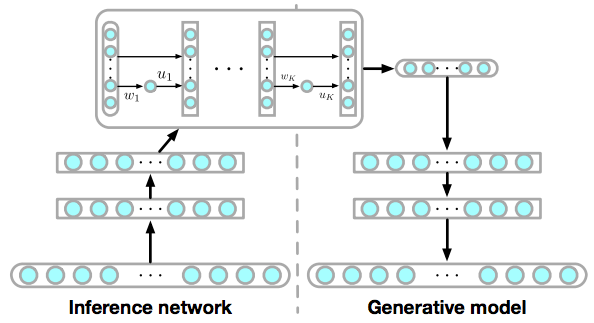
\includegraphics[width=0.6\textwidth]{NormFlowDiagram.png}
\caption{VAE with normalizing flow --- flow diagram, from \cite{RM15}.}
\label{fig:VAENormFlow}
\end{center}
\vspace{-0.5em}
\end{figure}

Normalizing flow describes a series of transformations on the initial probability distribution.  These 
transformations are invertible mappings and at the end of the series, a new probability distribution is 
obtained.  The transformations, $f$, must be chosen such that they are smooth and invertible (i.e. 
$f^{-1} = g$, where $g(f(\bz)) = \bz$).  Also, if $\bz \sim q(\bz)$, then the transformed random variable, 
$\bz_1 = f(\bz)$, has the following distribution, $q(\bz_1)$:
\begin{equation}
	\bz_1 \sim q(\bz_1) = q(\bz) \left|\det\frac{\partial f}{\partial\bz}\right|^{-1}
\end{equation}

We can perform $K$ transformations to the initial random variable, $\bz_0$, to obtain the final random variable,
$\bz_K$, where:
\begin{equation}
	\bz_K = f_K(f_{K-1}( \,\cdot\cdot\cdot\, (f_2(f_1(\bz_0)))))
\end{equation}
\begin{equation} \label{eq:logqkzk}
	\log q_K(\bz_K) = \log q_0(\bz_0) - \sum_{k=1}^K \log \left|\det\frac{\partial f_k}{\partial\bz_{k-1}}\right|
\end{equation}

The transformations, $f$, that are used are of the form:
\begin{equation}
	f(\bz) = \bz + \bu \cdot h(\bw^\top\bz + b)
\end{equation}
where $\bu, \bw \in \R^D$, $b \in \R$, and $h$ is a smooth non-linearity that is at least once differentiable.
This is called a planar flow.  We use $h(\cdot) = \tanh(\cdot)$ and $h'(\cdot) = 1 - \tanh^2(\cdot)$ in our 
experiments.  Plugging this into Equation \ref{eq:logqkzk}, we get:
\begin{equation}
	\log q_K(\bz_K) = \log q_0(\bz_0) - \sum_{k=1}^K \log \left|1 + \bu_k^\top\psi_k(\bz_{k-1})\right|
\end{equation}
where $\psi_k(\bz) = h'(\bw^\top\bz + b)\bw$. With these equations, the function we want to minimize becomes:
\begin{equation} \label{eq:ELBO_NormFlow}
	\mathcal{F}(\bx) = \E_{q_0}\left[\log q_0(\bz_0)\right] - \E_{q_0}\left[\log p(\bx, \bz_K)\right] 
					- \E_{q_0}\left[\sum_{k=1}^K\log \left|1 + \bu_k^\top\psi_k(\bz_{k-1})\right|\right]
\end{equation}

\section{Related Work}
\label{sec:RelatedWork}
\citet{RM15} also introduce another type of flow called radial flow.  Radial flow differs from planar flow in the
transformation function, $f$.  The transformation is $f(\bz) = \bz + \beta\cdot h(\alpha, r)(\bz - \bz_0)$, where
$\alpha \in \R^+$ and $\beta \in \R$.  The changes to the initial distribution, $q_0$, differ between the two
transformation functions.  Planar flows apply contractions and expansions perpendicular to the hyperplane,
$\bw^\top\bz + b$, whereas radial flows apply contractions and expansions radially around $\bz_0$.

Inverse autoregressive flow, which is a part of the family of normalizing flows, was introduced by \citet{KS16}.
In this flow, the series of transformations is initialized by sampling $\bz_0 \sim q(\bz \given \bx)$, as before. 
Then, each successive $\bz$ is computed using the transformation: $\bz_t = \bmu_t + \bsig_t \odot \bz_{t-1}$,
where $t$ indexes the transformations.  After $T$ transformations, the log distribution becomes: 
$\log q(\bz_T \given \bx) = -\sum_{i=1}^D\left(\frac{1}{2}\epsilon_i^2 + \frac{1}{2}\log(2\pi) + \sum_{t=0}^T\log\sigma_{t,i}\right)$
The resulting log marginal probabilities proved to be larger than those computed using previous methods of
variational inference.

\citet{D16} introduce another type of transformation called the real-valued non-volume preserving (real NVP) 
transformation. Similar to normalizing flow, \citet{D16} propose an invertible transformation from a simple
latent distribution to a complex distribution of the form:
\begin{align}
	y_{1:d} &= x_{1:d} \\
	y_{d+1:D} &= x_{d+1:D} \odot \exp\left(s(x_{1:d})\right) + t\left(x_{1:d}\right)
\end{align}
Using this mapping as $f$ in Equation \ref{eq:logqkzk}, we can compute the determinant and 
obtain $\log q_K(\bz_K)$ accordingly. The difference between real NVP and normalizing flows is that 
real NVP only transforms a portion of the input, from dimension $d+1$ onwards, through the exponential 
of an affine linear transformation and element-wise multiplied with the input. They claim that the generated 
samples using this transformation performs better than autoregressive models such as PixelRNN.

\section{Results and Comparison}

\subsection{Overview}
We compared the performance of the two models on the MNIST dataset to see the effects of the normalizing
flow layers. We used the same model and hyperparameters to achieve a fair comparison. The only difference 
between the models is the training loss, $\mathcal{F}$, as presented in Section \ref{sec:FormalDescription}, 
and the addition of normalizing flow layers from the latent sample to the generator network. We created 3 
normalizing flow models, each with a different number of normalizing flow layers. The code for these experiments
can be found online\footnote{\texttt{https://github.com/blisc/CSC412-Project}}.

For each model, we trained them for 100 epochs of the dataset with the Adam optimizer. In order to approximate 
the expectations present in Equations \ref{eq:ELBO_VAE} and \ref{eq:ELBO_NormFlow}, we used Monte Carlo 
estimation with a single sample of the latent variables per data point. For the latent space, we chose to 
parameterize it as a 20-dimensional Gaussian with mean and diagonal covariance as determined by the 
recognition network. Table \ref{tab:hyperparameters} shows the various hyperparameters that were used to
train the models.

\begin{table}[htbp]
\centering
\caption{Table of hyperparameters used to train the VAEs.}
\label{tab:hyperparameters}
	\begin{tabular}{|c||c|c|c|c|}\hline
	\multirow{2}{*}{Models}    & \multirow{2}{*}{Baseline} & Normalizing & Normalizing & Normalizing \\
	                       &               &       Flow     &          Flow       &           Flow           \\\hline\hline
	%Number of Layers           & 0      & 3         & 5          & 8          \\\hline
	\multicolumn{5}{|c|}{\textbf{Training Hyperparameters}}			                  \\\hline
	Optimizer                  & \multicolumn{4}{|c|}{Adam with TensorFlow Defaults}                 \\\hline
	Learning Rate              & 0.001    & 0.001            & 0.001            & 0.001            \\\hline
	Batch Size                 & 128      & 128              & 128              & 128              \\\hline
	Training Epochs            & 100      & 100              & 100              & 100              \\\hline
	Latent Gaussian Dimensions & 20       & 20               & 20               & 20               \\\hline\hline
	\multicolumn{5}{|c|}{\textbf{Recognition Network}}                                                        \\\hline
	Hidden Layers              & 2        & 2                & 2                & 2                \\\hline
	Hidden Units               & 500      & 500              & 500              & 500              \\\hline
	Normalizing Flow Layers    & 0        & 3                & 5                & 8                \\\hline
	Hidden Units Activation    & ReLU     & ReLU             & ReLU             & ReLU             \\\hline
	Final Activation           & tanh     & tanh             & tanh             & tanh             \\\hline\hline
	\multicolumn{5}{|c|}{\textbf{Generator Network}}                                                          \\\hline
	Hidden Layers              & 2        & 2                & 2                & 2                \\\hline
	Hidden Units               & 500      & 500              & 500              & 500              \\\hline
	Hidden Units Activation    & ReLU     & ReLU             & ReLU             & ReLU             \\\hline
	Final Activation           & sigmoid  & sigmoid          & sigmoid          & sigmoid         \\\hline
	\end{tabular}
\end{table}

\subsection{Baseline (Vanilla) VAE}
After training the baseline VAE to the MNIST dataset, the negative variational bound of the model was computed
by averaging the loss across 10 samples of the latent space given each data point from the data set. The negative variational lower bound
was approximately 109.23. The training loss is shown in Figure \ref{fig:BaselineLoss}.

\begin{figure}[htbp]\hspace{-2.5em}
\begin{subfigure}{0.5\textwidth}
\begin{center}
	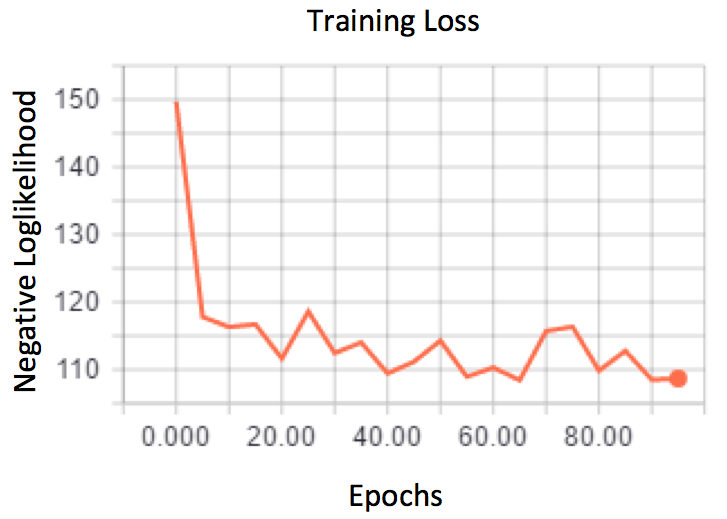
\includegraphics[width=0.9\textwidth]{BaselineLoss.png}
\caption{Loss curve for the vanilla VAE.}
\label{fig:BaselineLoss}
\end{center}
\end{subfigure}
\begin{subfigure}{0.5\textwidth}
\vspace{-2.3em}
\hspace{1em}
\begin{center}
	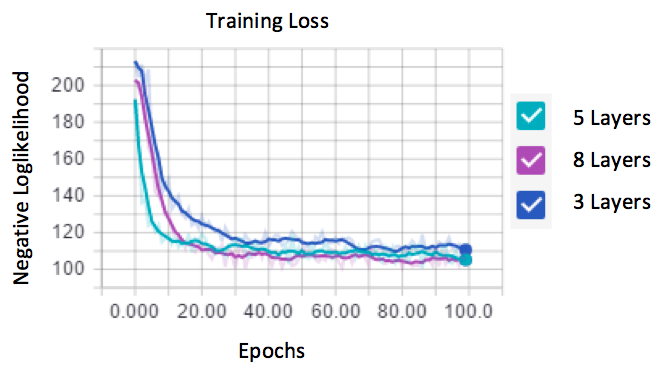
\includegraphics[width=1.2\textwidth]{NormFlowLoss.png}
\caption{Loss curve for the VAE with normalizing flows.}
\label{fig:NormFlowLoss}
\end{center}
\end{subfigure}
\caption{Loss curves for different VAE models.}
\vspace{-1em}
\end{figure}

\subsection{VAE with Normalizing Flow}
In the same manner as the baseline VAE, we approximated the log-likelihood using the lower bound
as stated in Equation \ref{eq:ELBO_NormFlow}. In order to evaluate the performance of the normalizing 
flow layers, we trained 3 models with 3, 5 and 8 normalizing flow layers to see how much of an impact 
these layers have. We obtained negative variational bound values of 111.96, 105.09 and 107.67 respectively.  
The training loss for all 3 models is shown in Figure \ref{fig:NormFlowLoss}.


\subsection{Model Comparison}
Comparing the variational bound values of the 4 models, we see that the model with 8 normalizing flow layers 
performs the best, followed by the model with 5 layers. An interesting observation is that the model with 
3 normalizing flows layers performs worse than the baseline model. We expected that the normalizing flows 
would have been able to better approximate the posterior than a model without those layers.

Figures \ref{fig:SampleBaseline}, \ref{fig:NormFlow35} and \ref{fig:NormFlow8} show the reconstructions 
produced by each model. We took the first 100 images from the MNIST training set and plot their reconstruction. 
Qualitatively, it seems that the baseline model produces the sharpest images whereas the normalizing flow 
models produce blurrier images. This is the opposite of what we expected given the variational bounds discussed
previously. However, because the loss functions for the two models are slightly different, the lower bound might 
not be the best measurement of image quality.

\begin{figure}[htbp]
\begin{subfigure}{0.5\textwidth}
\begin{center}
	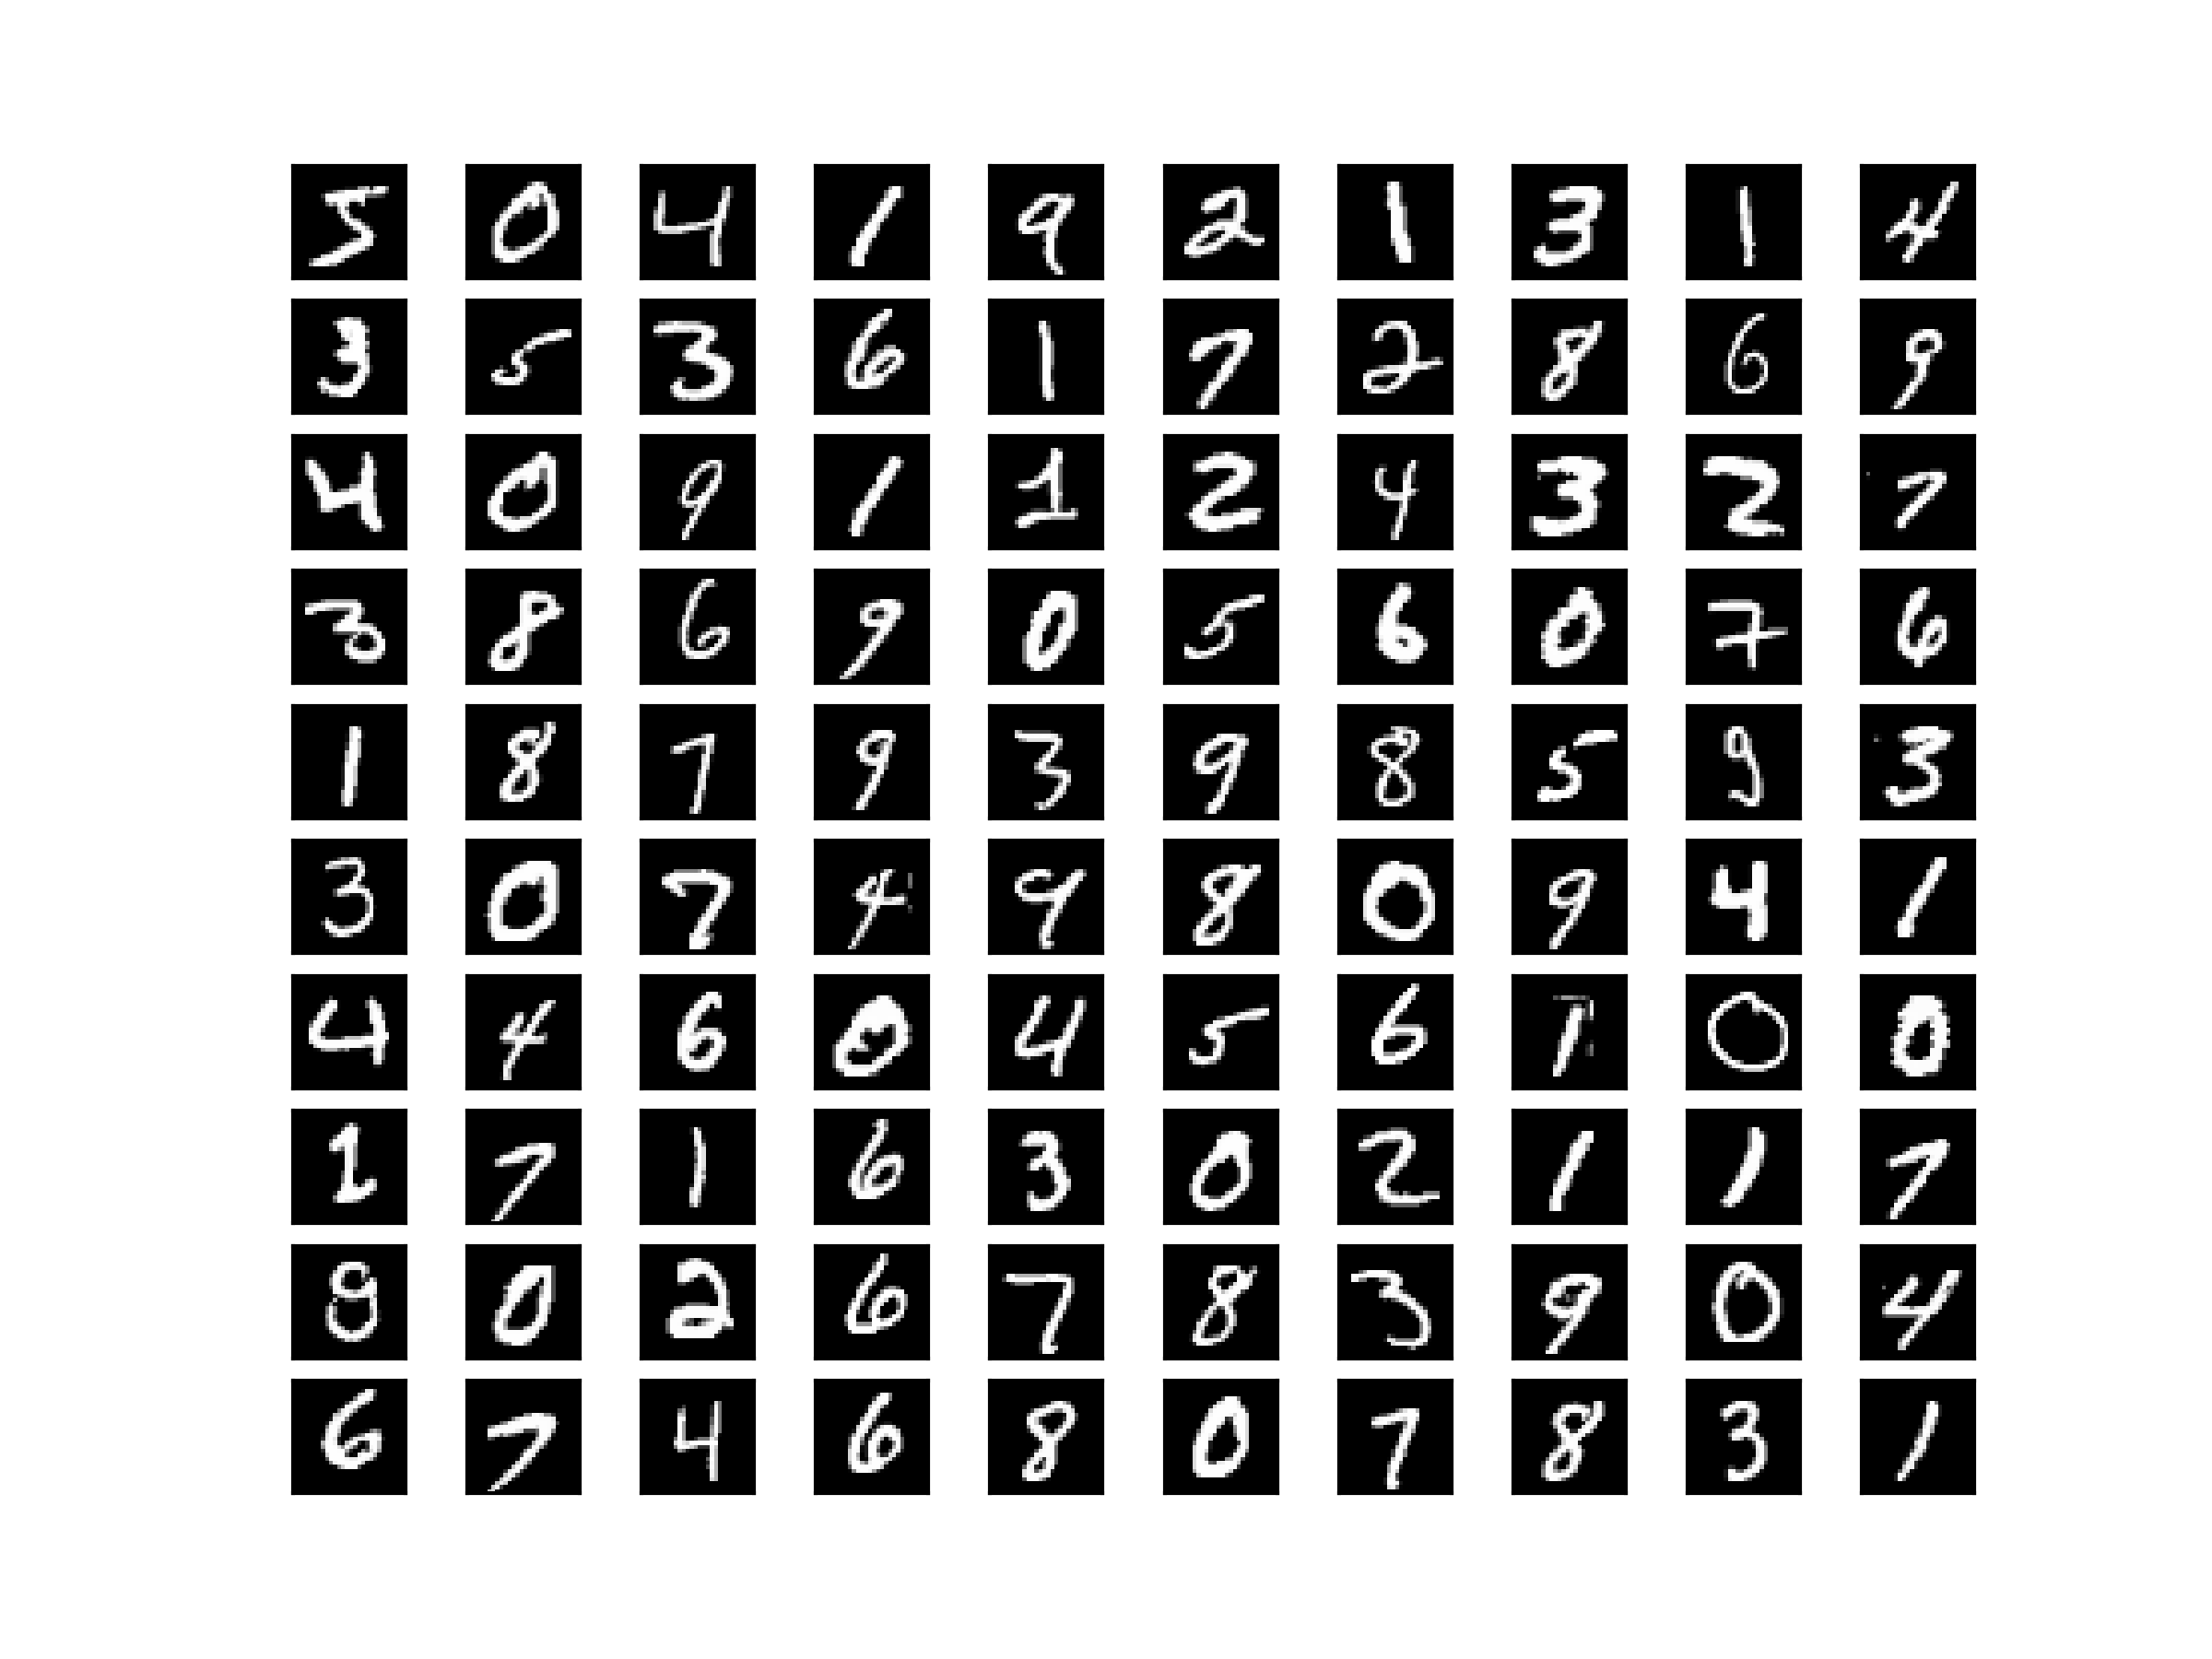
\includegraphics[width=\textwidth]{Samples.png}
\caption{Input images from MNIST dataset.}
\label{fig:samples}
\end{center}
\end{subfigure}
\begin{subfigure}{0.5\textwidth}
\begin{center}
	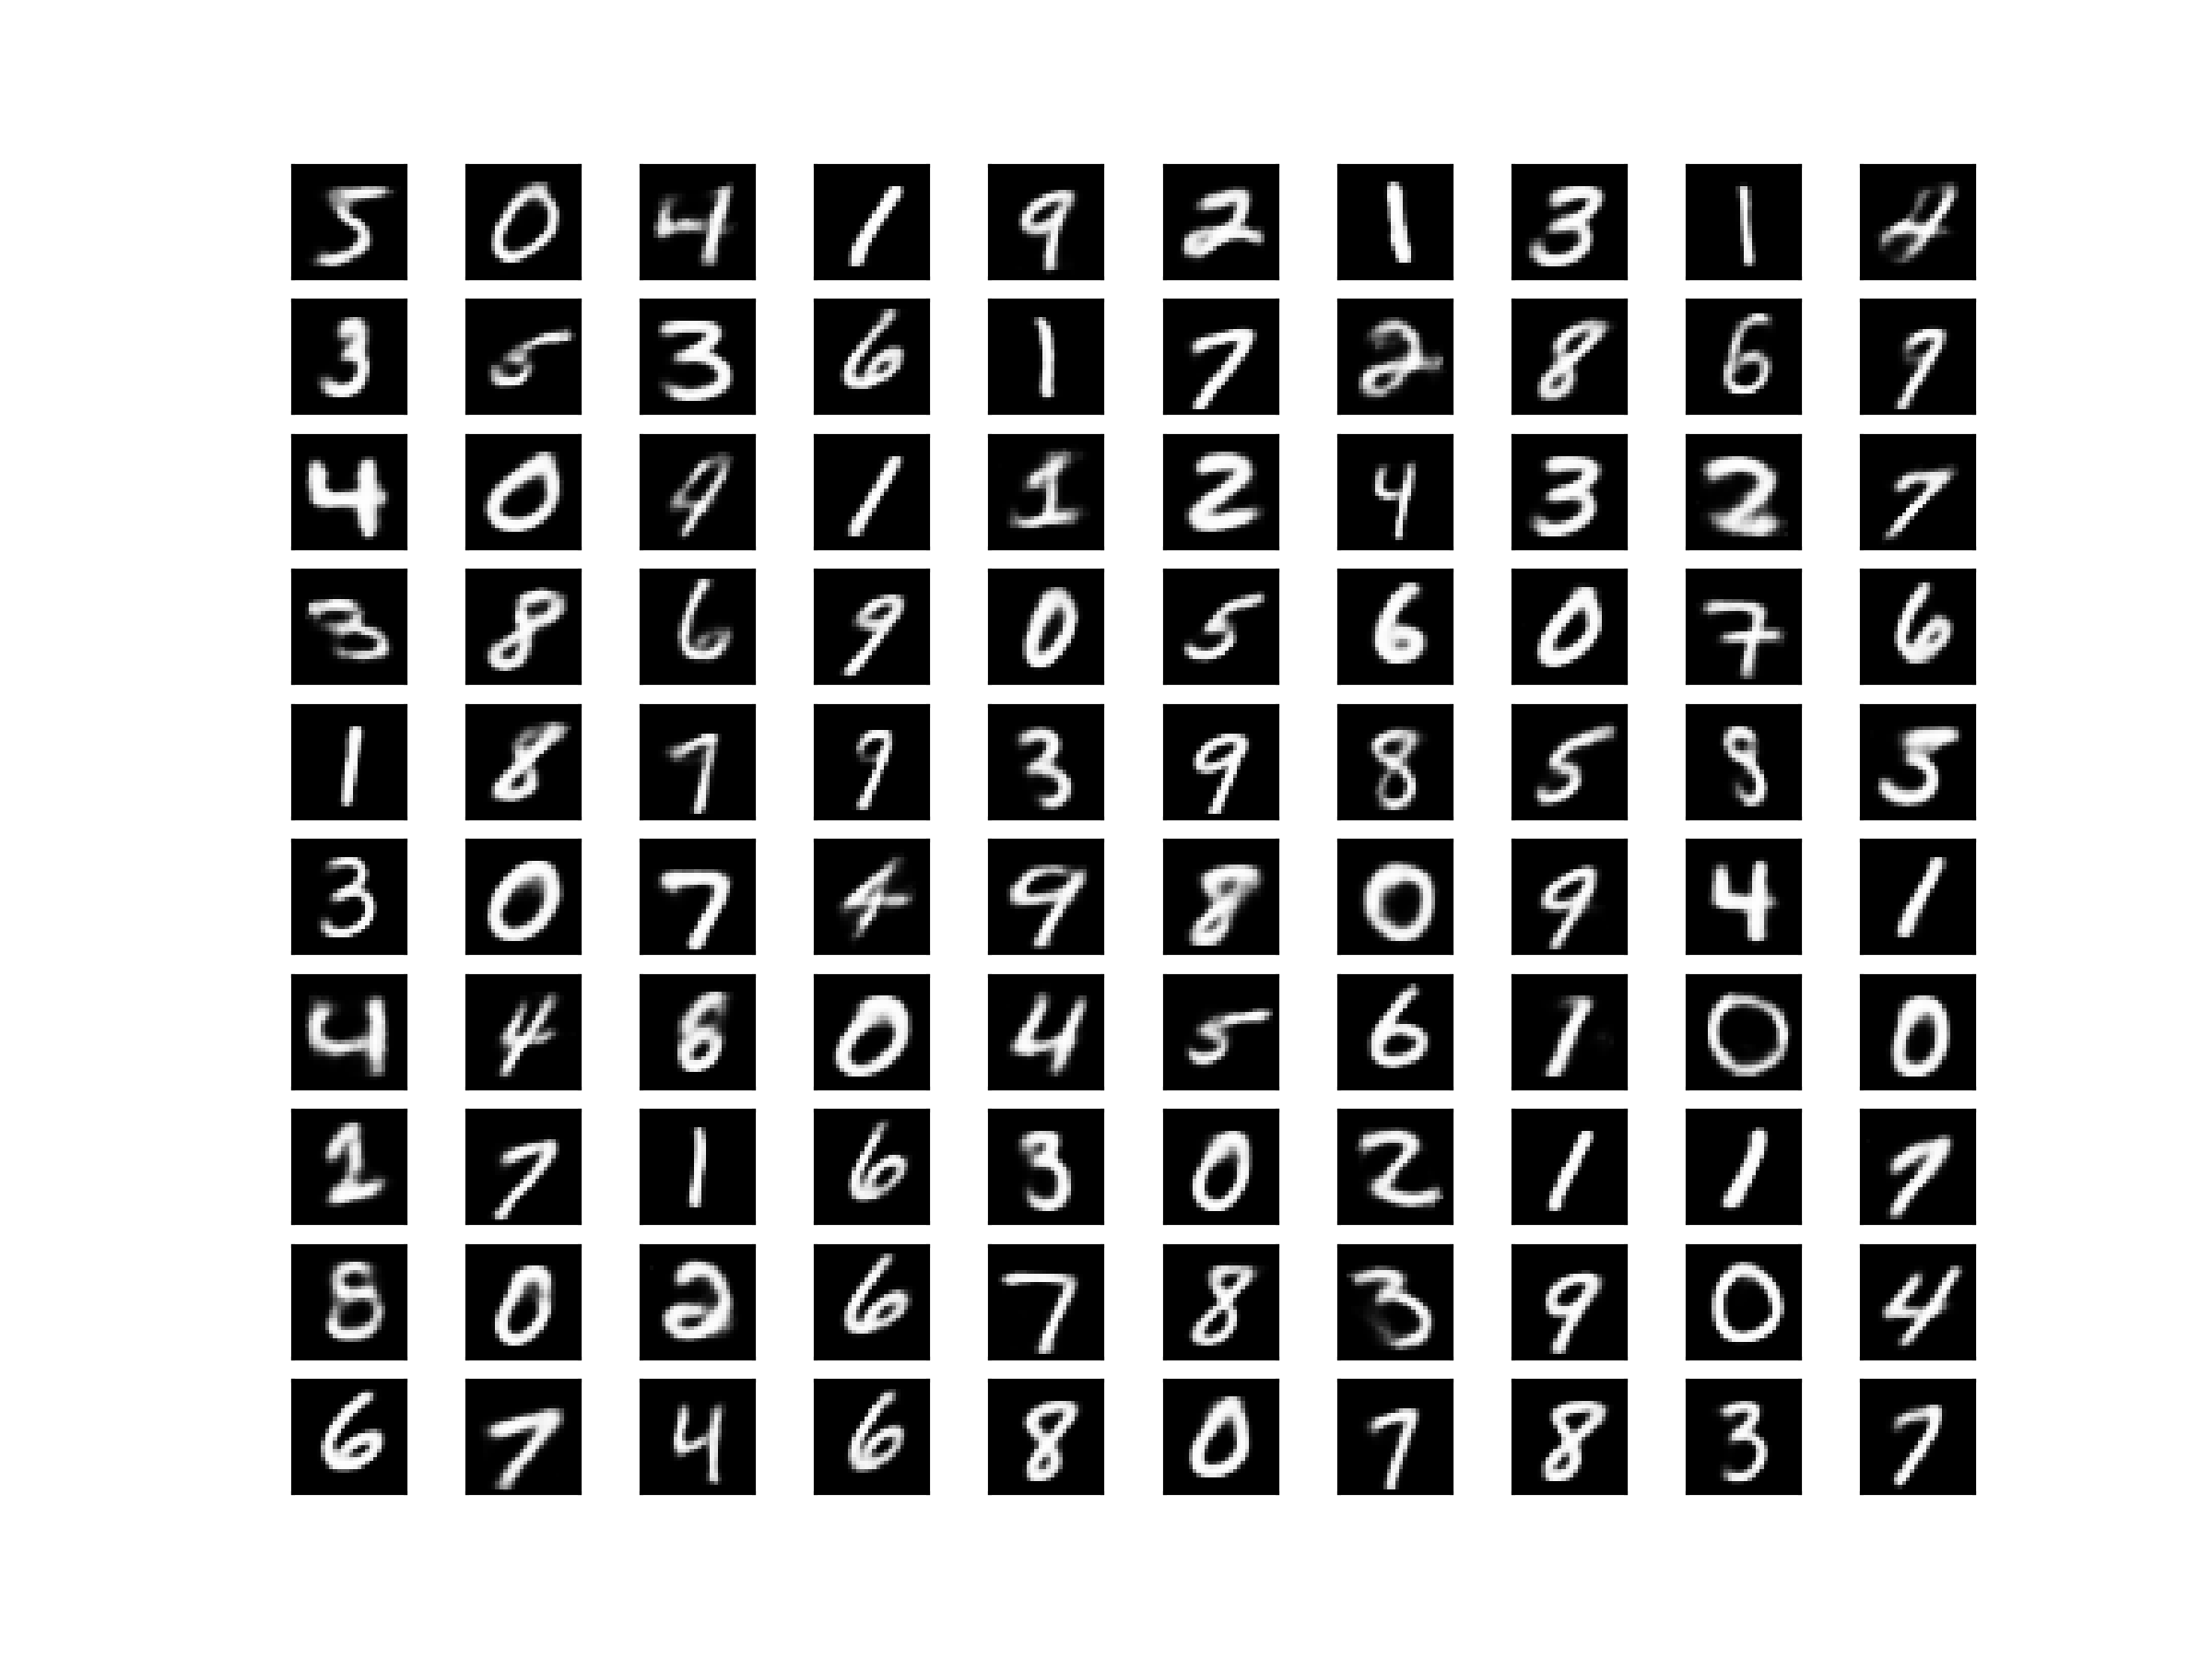
\includegraphics[width=\textwidth]{reconstruction_Baseline.png}
\caption{Reconstructed images using the vanilla VAE.}
\label{fig:BaselineReconstruction}
\end{center}
\end{subfigure}
\caption{Training images and reconstructed images using the vanilla VAE.}
\label{fig:SampleBaseline}
\end{figure}

\begin{figure}[htbp]\hspace{-0.25em}
\begin{subfigure}{0.5\textwidth}
\begin{center}
	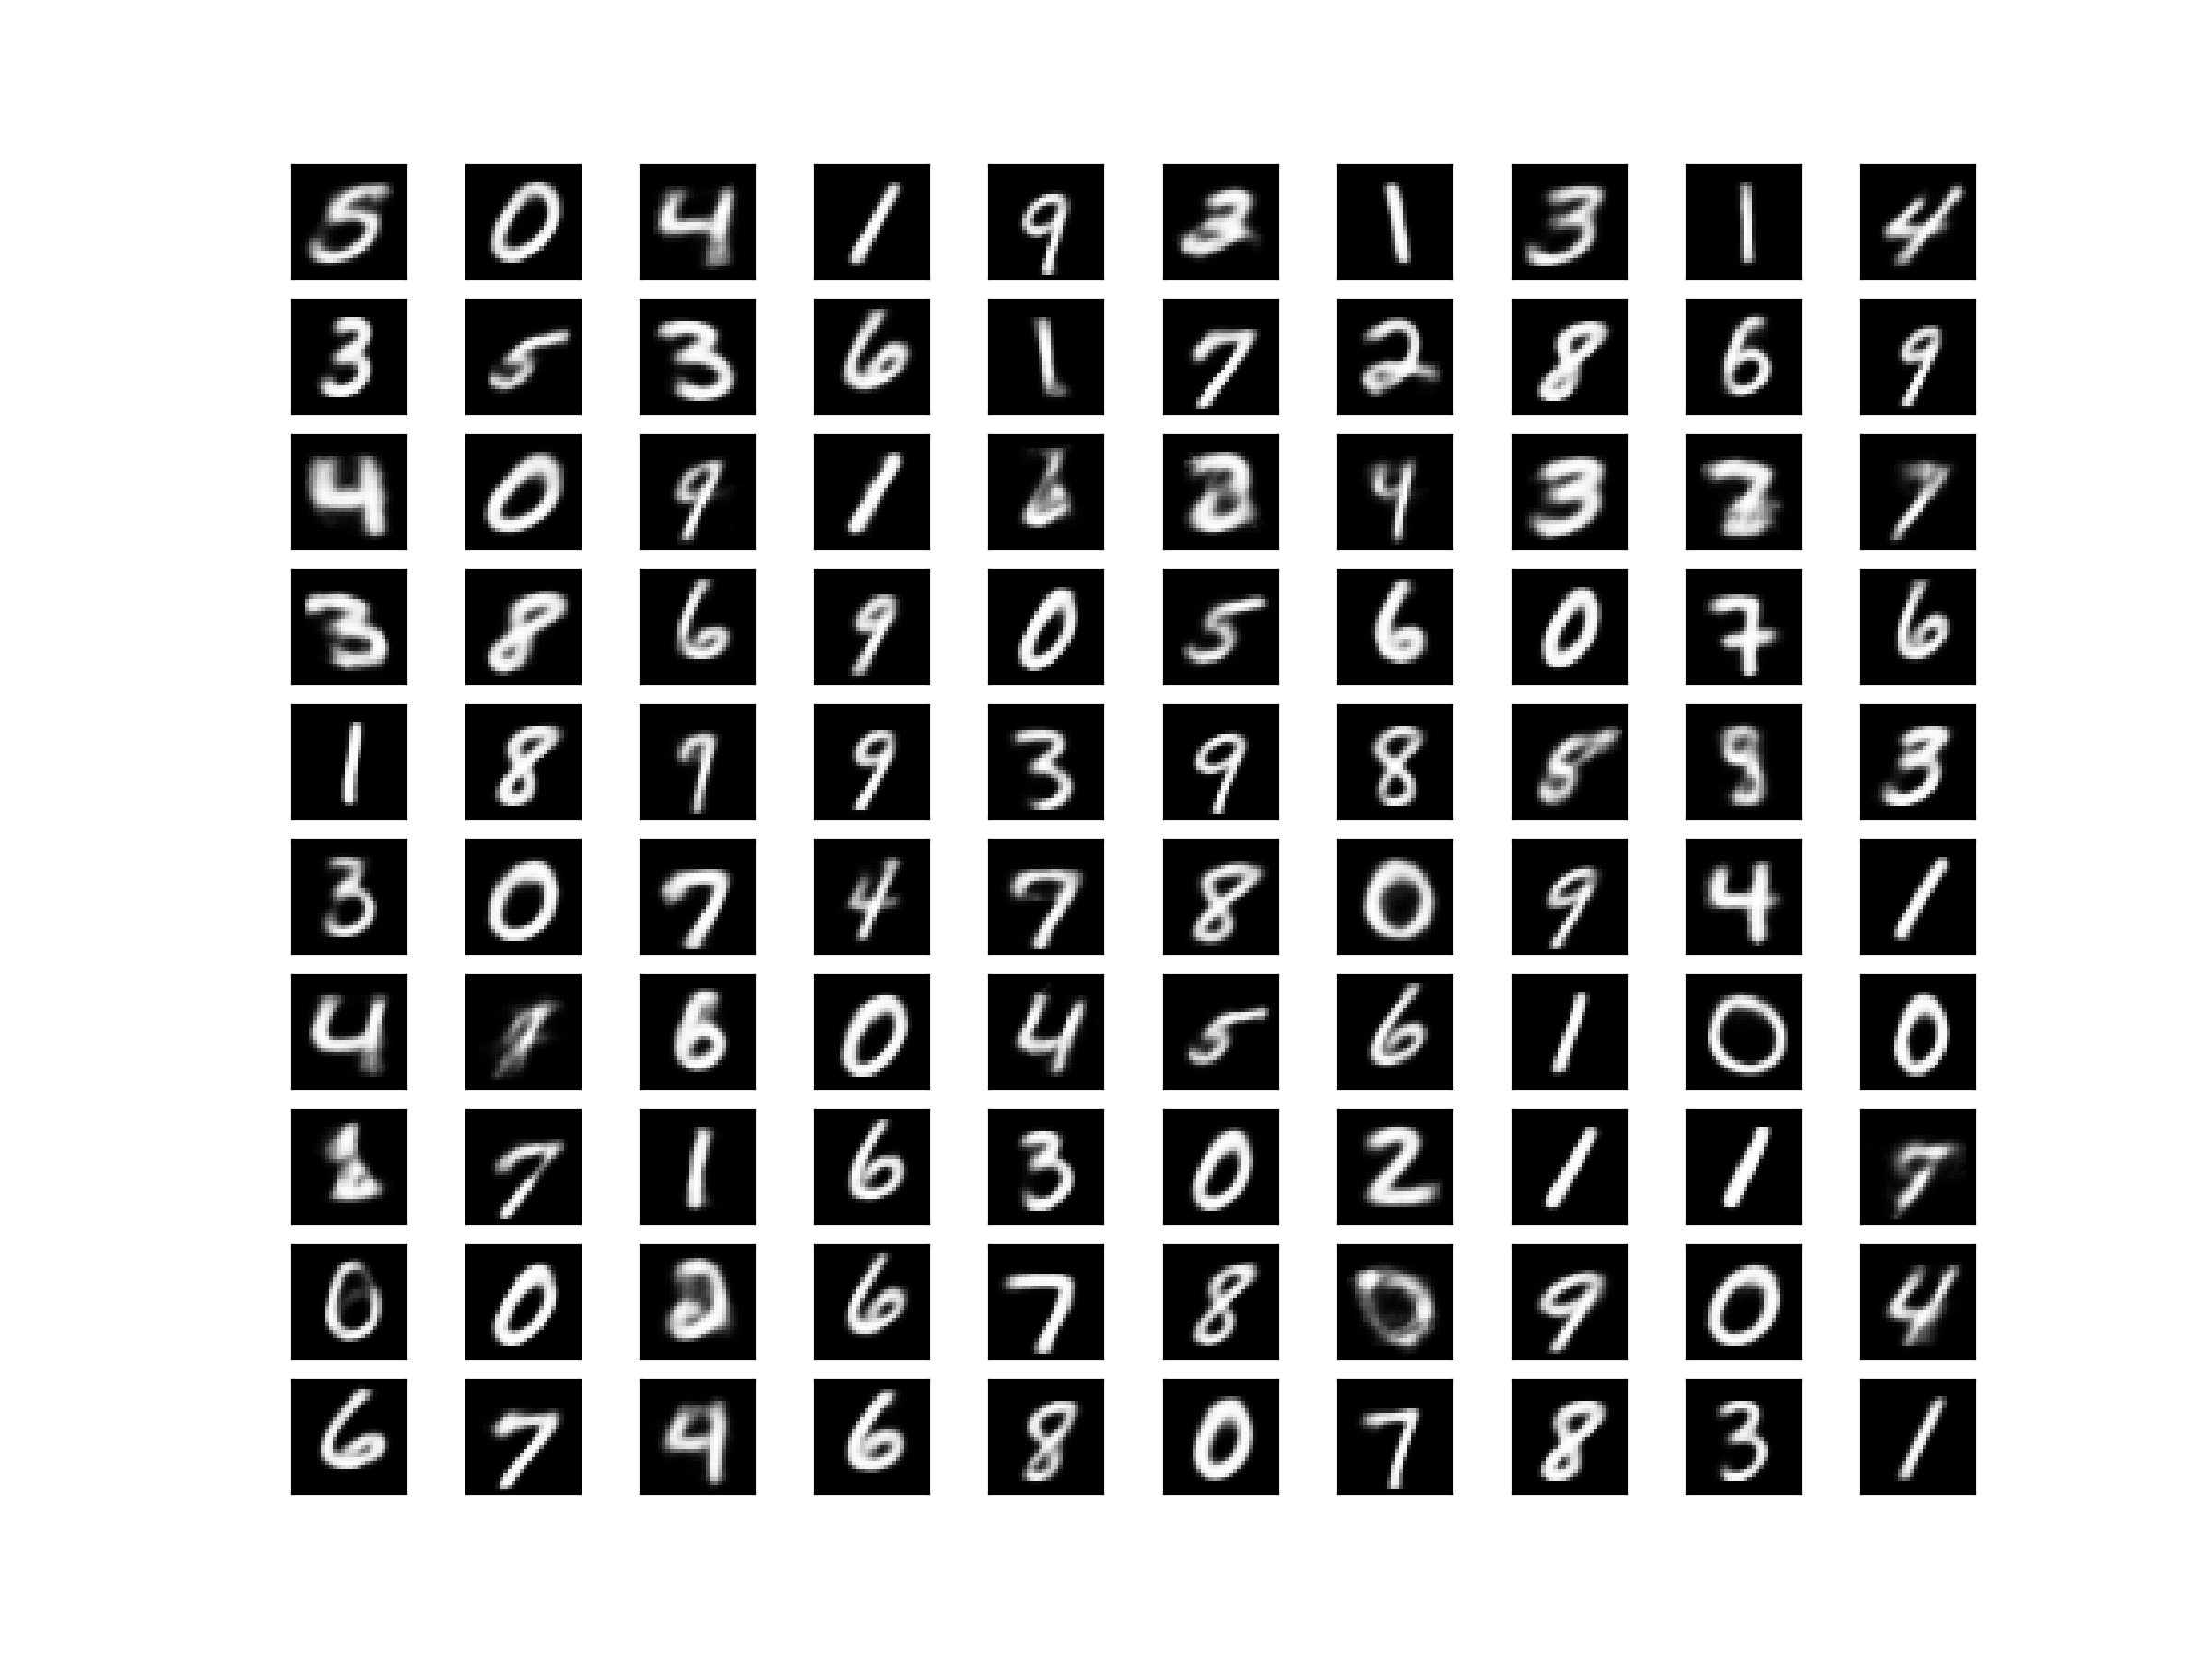
\includegraphics[width=\textwidth]{reconstruction_3Layers.png}
\caption{Reconstructed images using the VAE with 3 normalizing flow layers.}
\label{fig:NormFlow3}
\end{center}
\end{subfigure}\hspace{0.5em}
\begin{subfigure}{0.5\textwidth}
\begin{center}
	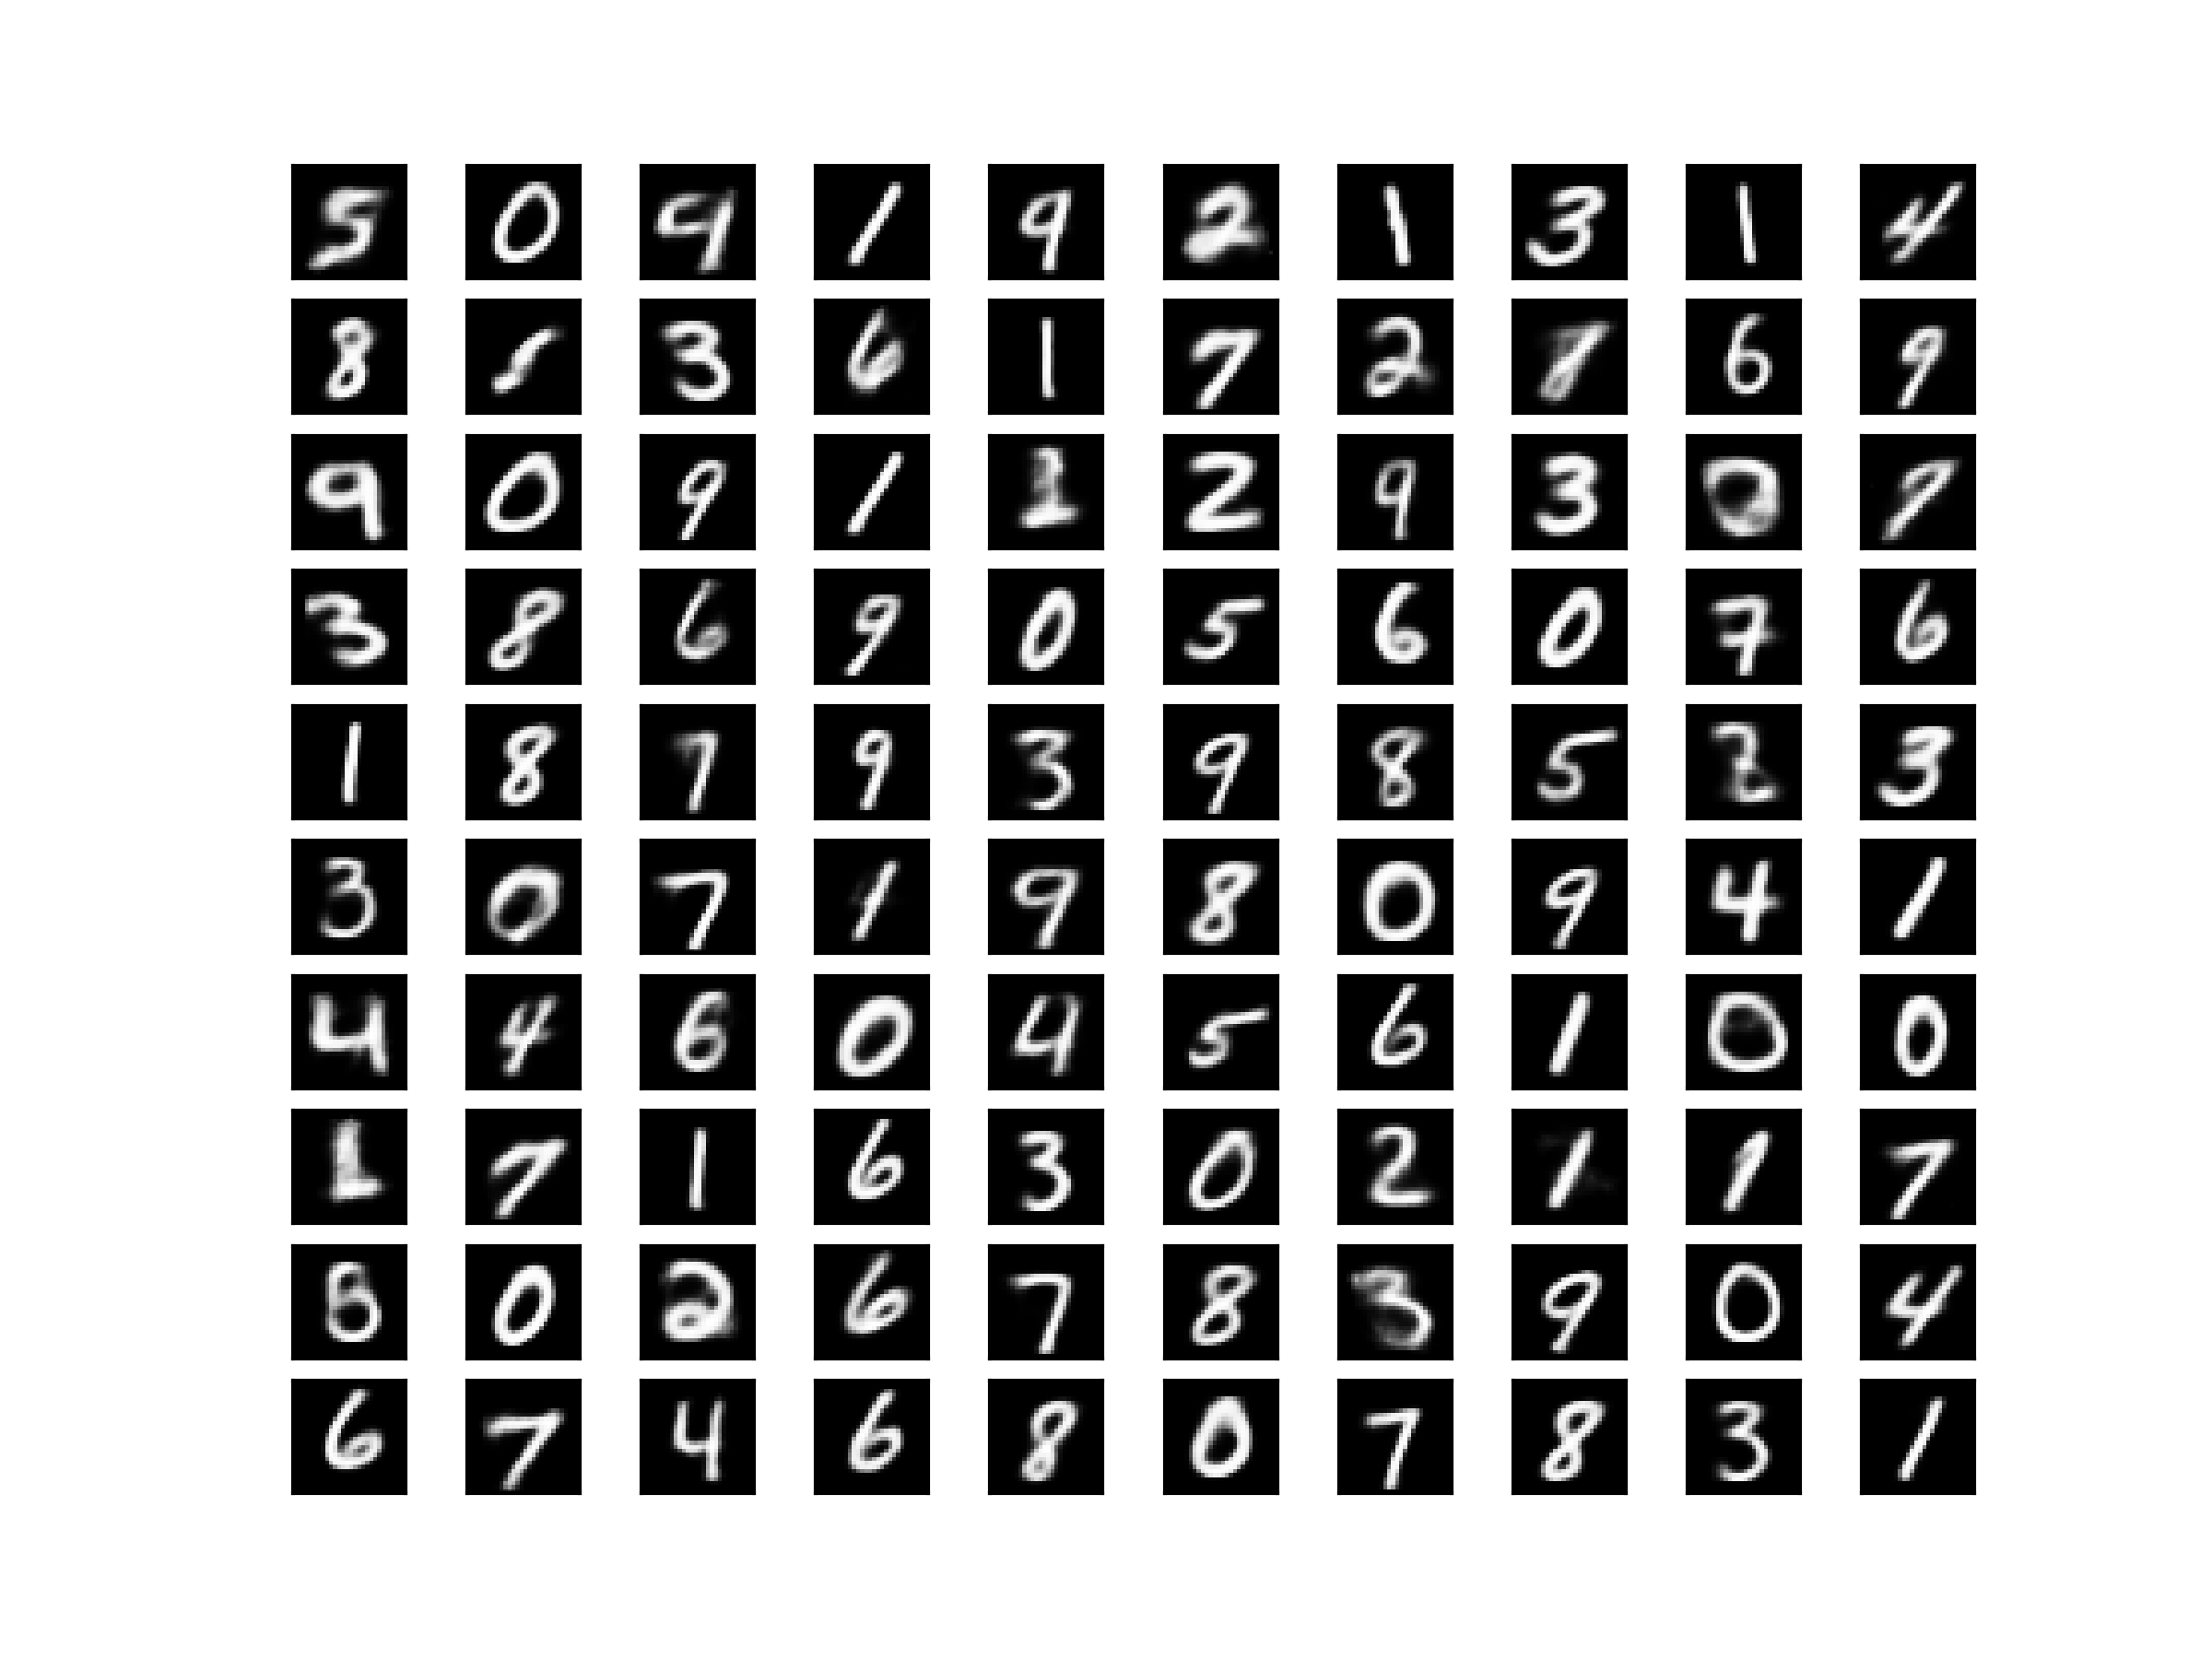
\includegraphics[width=\textwidth]{reconstruction_5Layers.png}
\caption{Reconstructed images using the VAE with 5 normalizing flow layers.}
\label{fig:NormFlow5}
\end{center}
\end{subfigure}
\caption{Reconstructed images using the VAE with 3 and 5 normalizing flow layers.}
\label{fig:NormFlow35}
\end{figure}

\begin{figure}[htbp]
\begin{center}
	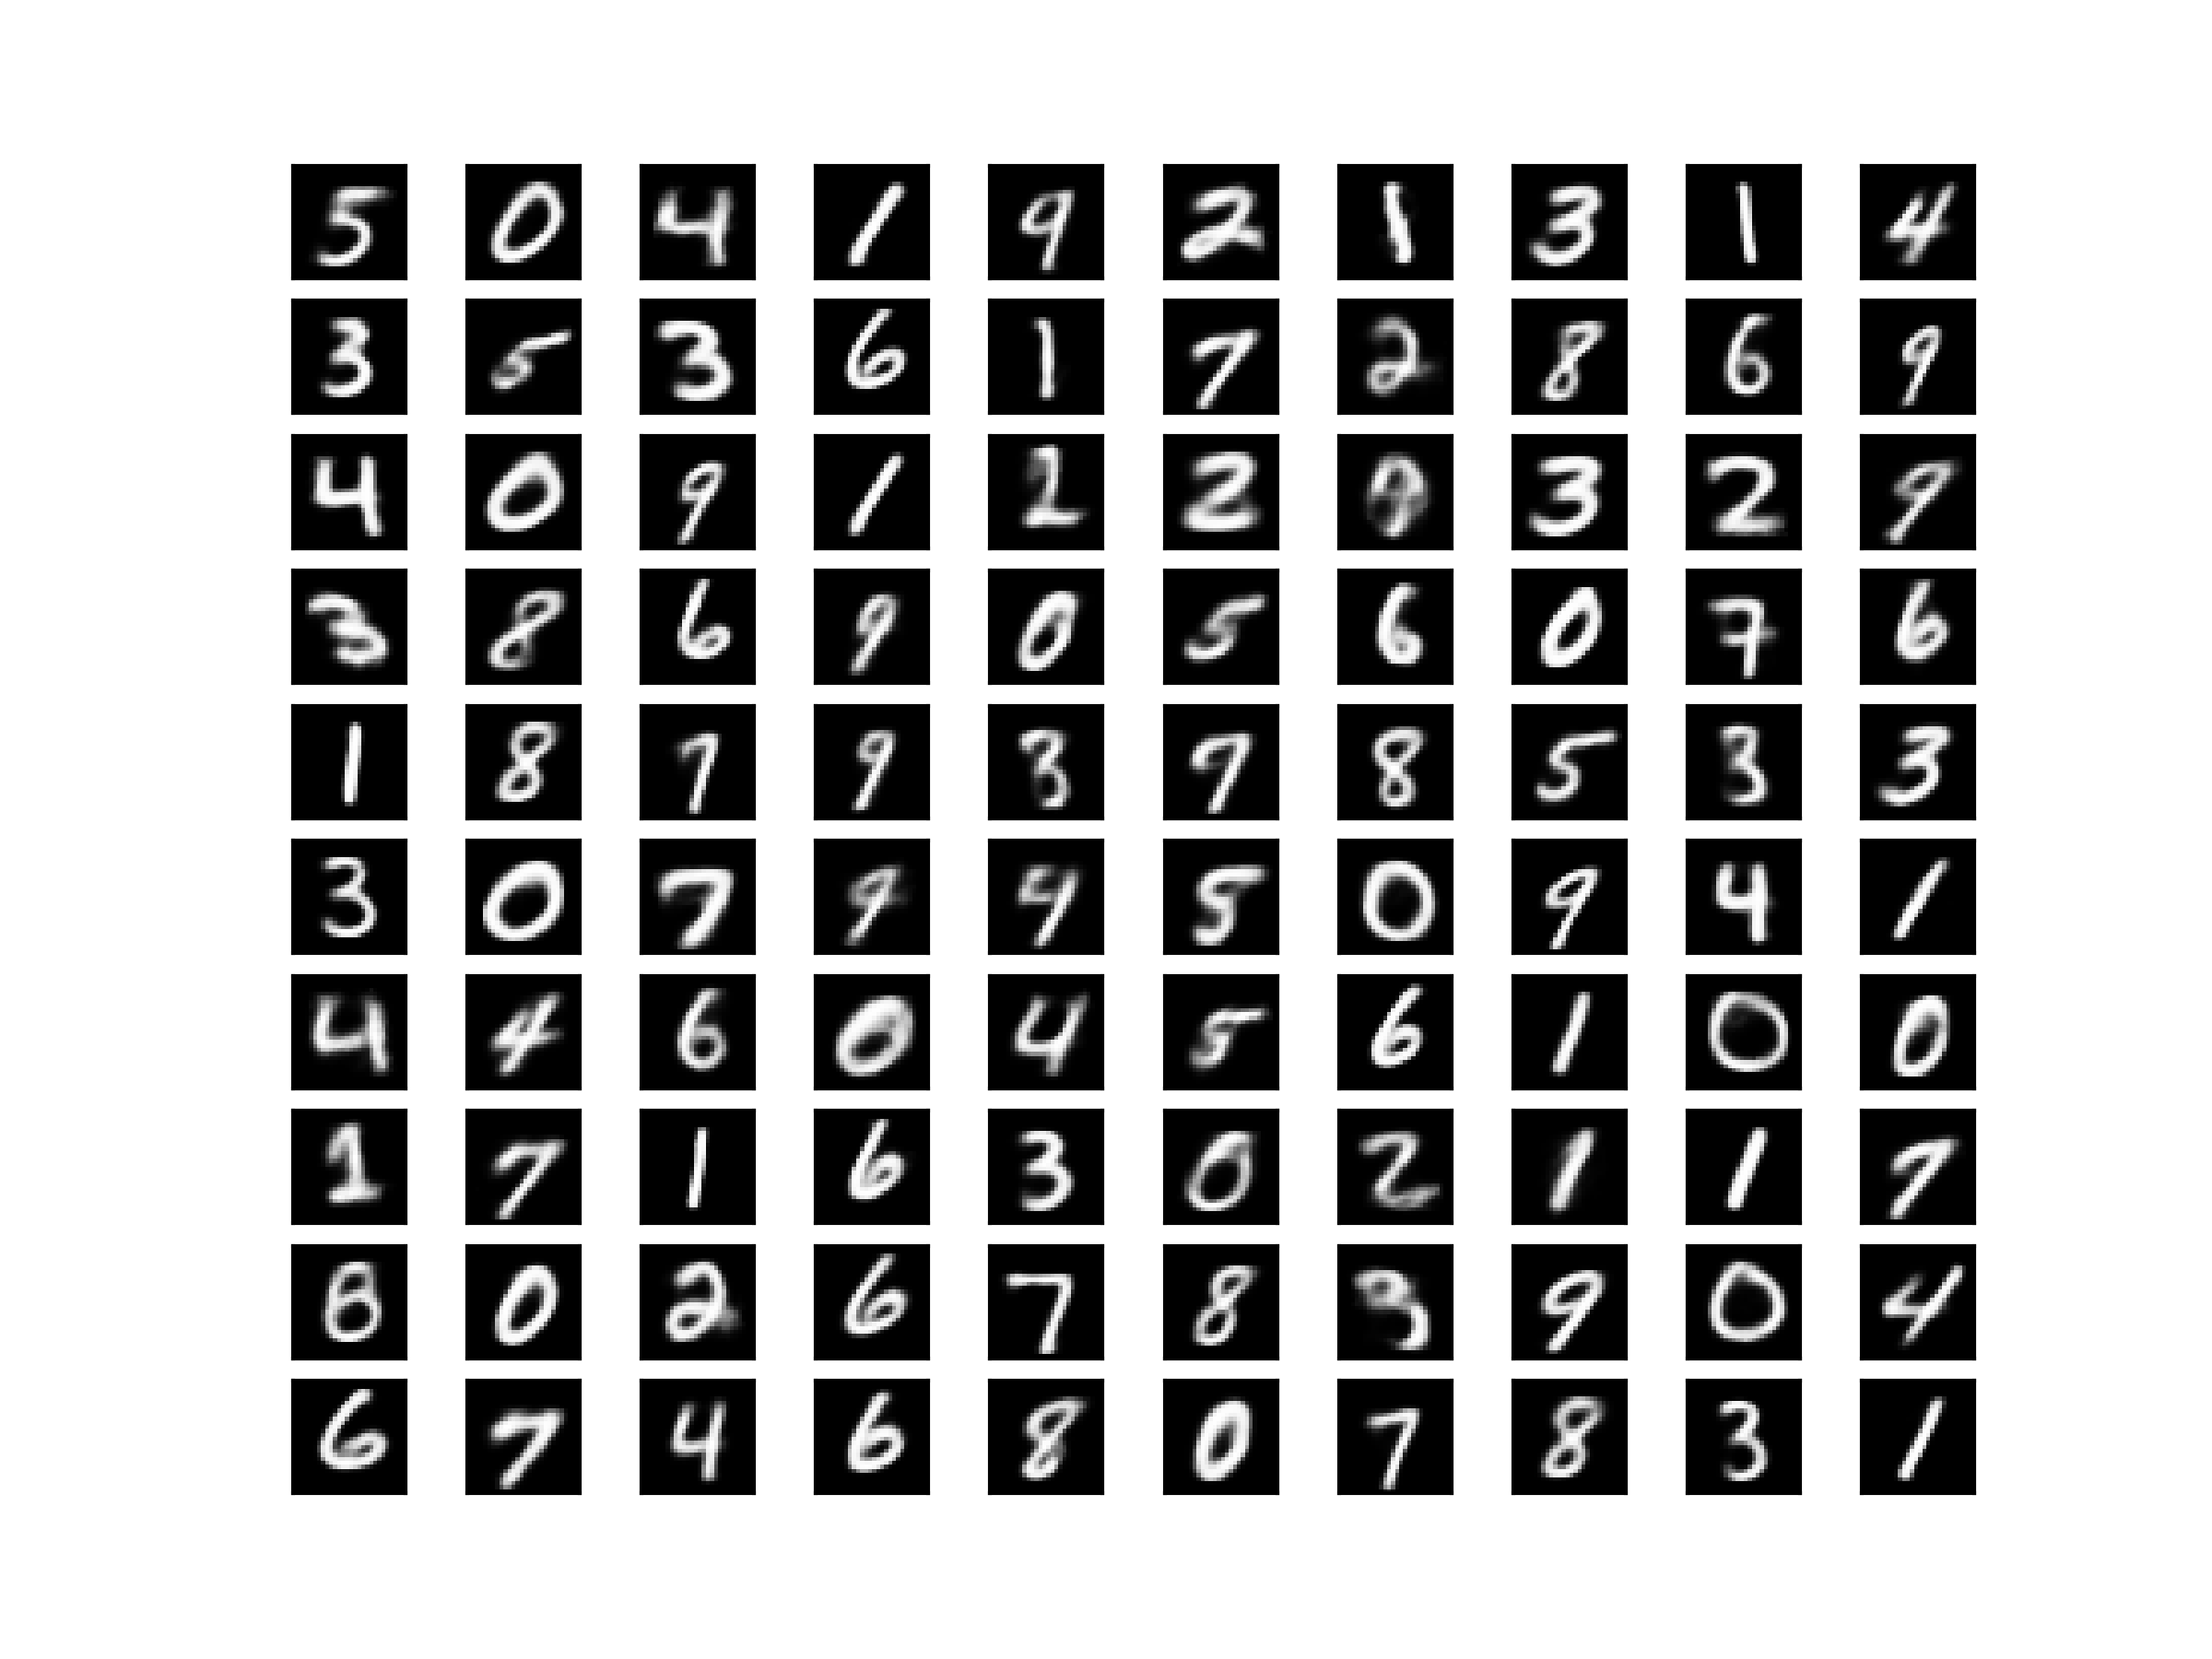
\includegraphics[width=0.52\textwidth]{reconstruction_8Layers.png}
\caption{Reconstructed images using the VAE with 8 normalizing flow layers.}
\label{fig:NormFlow8}
\end{center}
\end{figure}

\section{Limitations and Future Work}
Our original goal was to explore the difference between vanilla VAEs and normalizing flow VAEs. As we
explained in Section \ref{sec:FormalDescription}, normalizing flows should allow for more complex posteriors 
to be approximated and give our model more expressive power. However, as can seen from the qualitative 
samples, the addition of these normalizing flow layers does not always make our generator perform better. 
Perhaps one limitation of our review was the size of the model that we used. In \citet{RM15}, they trained a 
model with 40 latent dimensions and up to 80 normalizing flow layers. In the interest of time, our models were 
much smaller. This decision might have limited the complexity of our posterior. Another issue might be 
due to the added complexity of the normalizing flow layers. It might have required more training iterations 
for the normalizing flow models to fully converge in comparison to the baseline model. Perhaps, training 
the normalizing flow models for longer might yield better results.

Another limitation of the normalizing flow models is that while they increase the complexity of the posterior, 
the authors only provide an empirical result to show that normalizing flow models can learn arbitrary 
complex distributions. While these transformations help construct more complex posterior distributions, 
there is no proof that these models can learn any type of posterior distribution. Thus, we are still stuck 
with an approximation of the true posterior.

In Section \ref{sec:RelatedWork}, we presented three other transformations that can be applied. 
A good next step to expand the review would be to try these transformations as well to see if they 
result in better generated images. If we had more time and computing resources, it would be a good 
idea to test some of the presented limitations by increasing model complexity and training the model 
for more epochs.

\section{Conclusions}
In our work, we described two models of VAEs: vanilla VAEs and VAEs with differing numbers of
normalizing flow layers.  We compared the training loss among the the different VAE models and found
that the model with the greatest number of normalizing flow layers performed the best quantitatively.  
This is what we expected since normalizing flow layers allow for greater expressivity in the posterior 
approximation. Therefore, by introducing various transformations to a simple initial posterior distribution, 
more complex posterior distributions can be approximated. However, it is worth noting that the generated 
samples produced by the normalizing flow models are more blurry than those from the vanilla VAE 
indicating possible limitations in our review.


\small
%\bibliographystyle{IEEEtranN}
\bibliographystyle{plainnat}
\bibliography{references.bib}


\end{document}